\documentclass{article}
\usepackage[pdftex]{graphicx}
\usepackage{epstopdf}
\usepackage{fullpage}


\begin{document}
  \begin{center}
    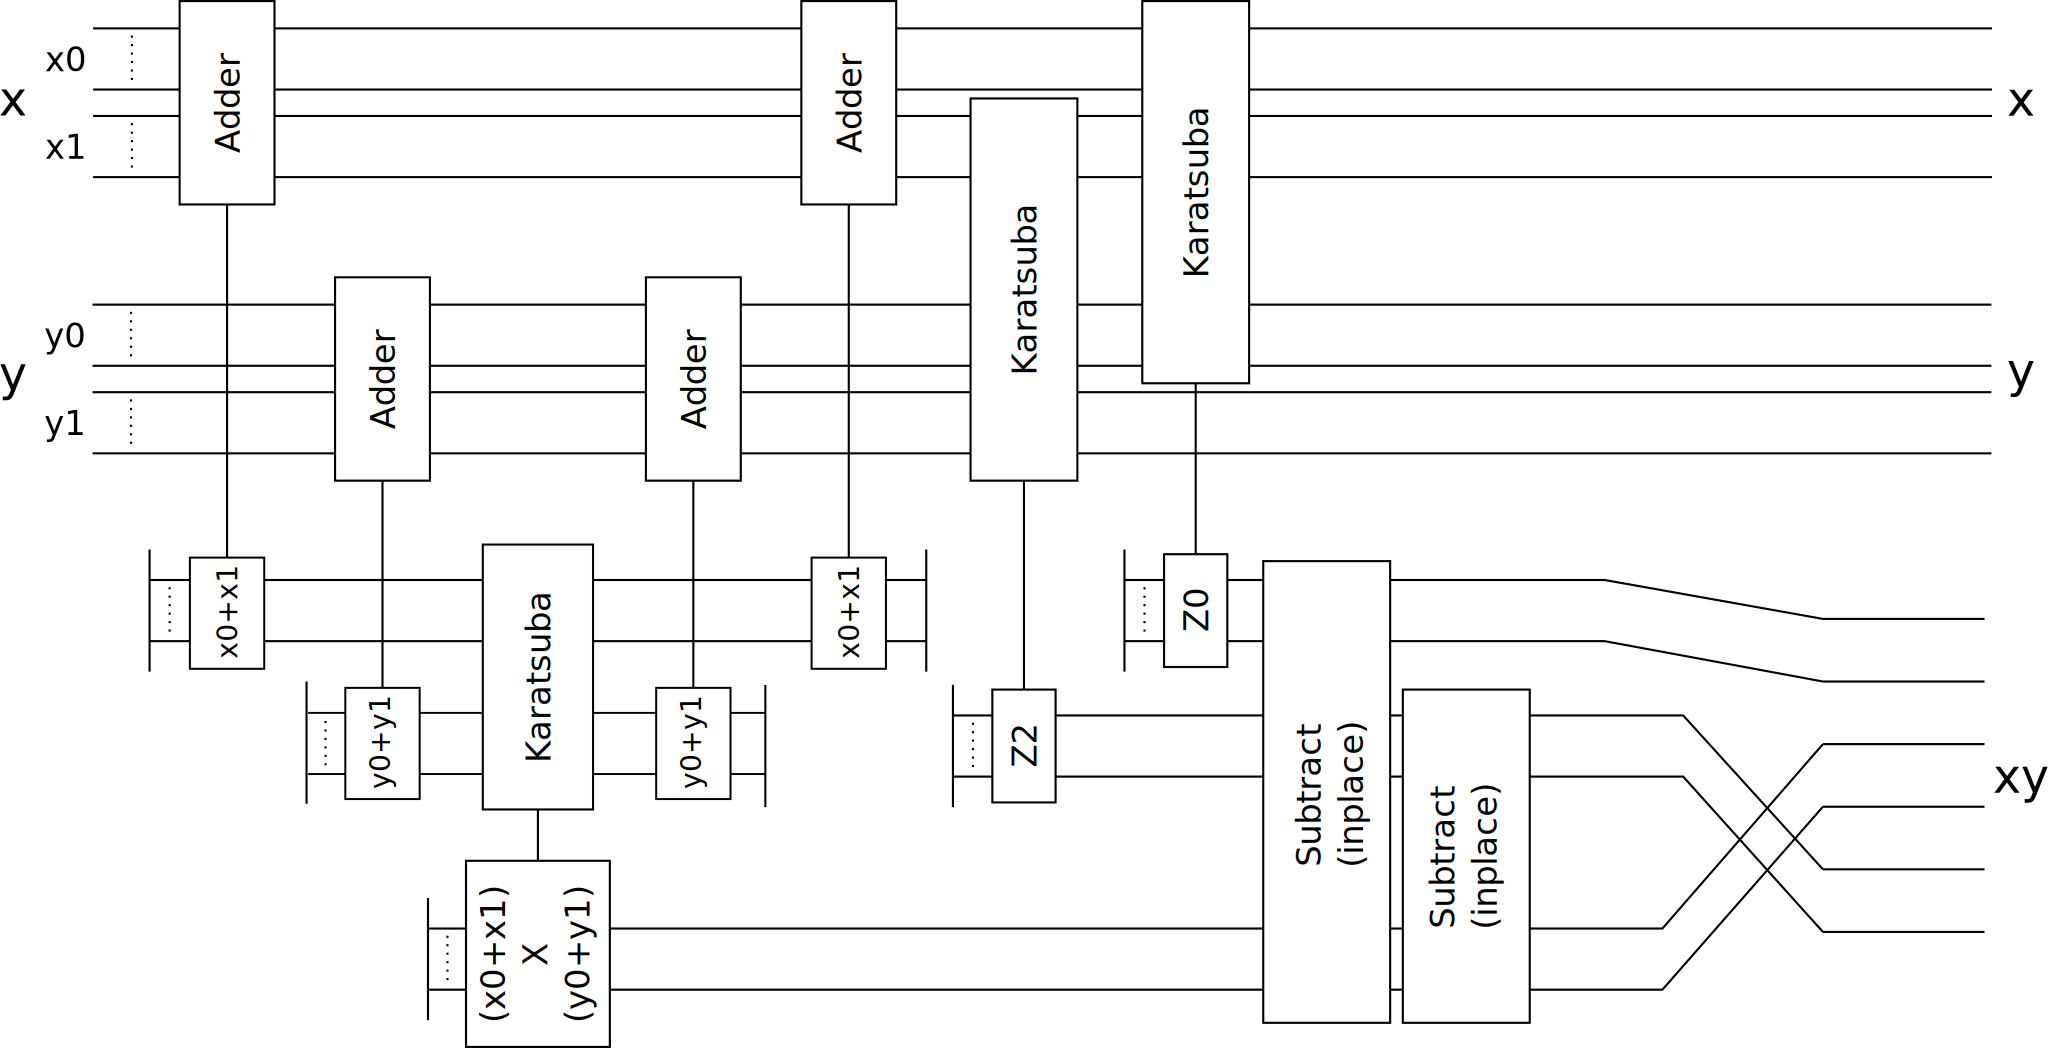
\includegraphics[scale=0.24]{karatsubaDiagram} 
  \end{center}

  Define the following gate counts for circuits of size $n$:
  \begin{itemize}
   \item $A_n$: out of place adder 
   \item $S_n$: in place subtractor 
   \item $K_n$: simple muliclication
  \end{itemize} 
  Also define $b$ as a cutoff level for karasuba recursion \\
  The number of gates in a Katatsuba circuit $K_n$ is given by:
  \[ K_n = 3^bM_{n/2^{b+1}} + \sum_{a=0}^{b} 3^a\left( 4A_{n/2^{a+1}} + 2S_{n/2^{a+1}}  \right)  \] 
	Note that in the above circuit all 3 Katasuba recursions can be done in parallel.

\end{document}
